\documentclass[journal, a4paper]{IEEEtran}

\usepackage{graphicx}
\usepackage{caption}
\usepackage{subcaption}
% some very useful LaTeX packages include:

%\usepackage{cite}
\usepackage{graphicx}
\usepackage{amsmath,eqparbox,booktabs,xparse}
\usepackage{smartdiagram}
\usetikzlibrary{quotes}
%\usepackage{psfrag}   
%\usepackage{subfigure}
\usepackage{neuralnetwork}
\usepackage{url}        % Written by Donald Arseneau
%\usepackage{stfloats}  % Written by Sigitas Tolusis
\usepackage{xcolor}
%\interdisplaylinepenalty=2500
\usepackage{listings}

\lstset{basicstyle=\ttfamily, keywordstyle=\bfseries}
\usetikzlibrary{arrows.meta, positioning}
\tikzset{%
    block/.style = {draw=gray, rectangle, thick,
        minimum height=6em, text width=4em, align=center}
}

\makeatletter
\NewDocumentCommand{\eqmathbox}{o O{c} m}{%
  \IfValueTF{#1}
    {\def\eqmathbox@##1##2{\eqmakebox[#1][#2]{$##1##2$}}}
    {\def\eqmathbox@##1##2{\eqmakebox{$##1##2$}}}
  \mathpalette\eqmathbox@{#3}
}
% Your document starts here!
\begin{document}

% Define document title and author
	\title{Project 1 of Deep Learning\\ \textit{\Large{Classification, weight sharing, auxiliary losses}}}
	\author{Francis \textbf{Damachi} - Costanza \textbf{Volpini}}
	\markboth{Project 1 - Deep Learning EE559 - EPFL}{}
	\maketitle
	
\begin{abstract}
The aim of this project was to show the impact of weight sharing and the use of auxiliary loss. The task was to compare two digits in a two-channel image. Starting from linear model until some more complex non-linear model, we have found out that convolutional neural networks represents the best solution to classify images.
\end{abstract}

\section{Introduction}
\label{sec:intro}
\textit{Convolutional neural network} (CNN) represents the most powerful model to analyse images. Indeed, CNN uses the pixel locality to learn better. 

We have started the project training simple linear models, in particular \textit{Linear Regression} and \textit{Logistic Regression} (see Section \ref{sec:linearmodel}) but we have notice that these models are too simple and not consider the pixel locality. We have then used a more complex model \textit{Neural Network} with one-loss and two-losses (as explained and showed in Section \ref{sec:nnmodel}), we got a bad accuracy caused by the fact that we have a model composed by just linear layer. The last model that we have implemented is the \textit{Convolutional neural network}, with this model we got a very good approximation (see Section \ref{sec:cnnmodel}).
In all the models, we have used \textit{Adam's method} instead of \textit{stochastic gradient descent} as optimizer since it use an adaptive learning rate (the learning rate of SGD has an equivalent type of effect for all the weights/parameters of the model \cite{reference0}).
As criterion, we have used \textit{Mean Square Error} for all the models.

For all the models we have explicitely separated in the code the feature extractor, used to process the input and extract high level features, from classifier(s), a simple linear layer that we have used to classify.

Section \ref{sec:data} explain the structure of the dataset, Section \ref{sec:codestruc} describes briefly the content of each file. In Section \ref{sec:comparison}, \ref{sec:conclusion} we have showed the performance accuracy obtained by each model with a fixed seed, explaining why we got these results.


\section{Data}
\label{sec:data}
The data set consists of an input series of $2\times14\times14$ tensor (2 images in grayscale). Training and test set is $1000$ pairs each. In total we will have six tensors: images ($N\times2\times14\times14$), prediction (boolean), classes of the two digits ($N\times2$), both for training and test sets. The MNIST database is composed by handwritten digits (from $0$ to $9$); to load the dataset we have used the provided function \texttt{generate\_pair\_sets(N)}.

\section{Code structure}
\label{sec:codestruc}
In this section contains the description of each file.
\begin{itemize}
    \item \texttt{scripts/data.py}: class to generate the dataset. Contains different methods (e.g. flat the input, get a dataset in 2D or in 3D, enable the hot-encoding).
    \item \texttt{scripts/model.py}: general class to define a model to train and test it (with corresponding plot and history).
    \item \texttt{scripts/models\_implemented.py}: contains all the model classes (e.g. NNModel1Loss, CNNModel2Loss).
    \item \texttt{main.py}: contains examples of each models, in order to call and train a model.
\end{itemize}

\section{Linear Models}
\label{sec:linearmodel}
We have implemented \textit{Linear Regression} and \textit{Logistic Regression}. Regression is represented by a final layer that it is linear. In the logistic regression we have used a sigmoid as an activation function in the output layer. A linear layer accept as input a vector of values, that is the reason why we need to flat the input (the raw input is composed by 2D images). In fact a linear layer give a weight to each pixel, then it will accept a vector composed by N rows and D dimensions (columns), in our case it will have size $14 \times 14 \times 2$. Linear layers bad generalize images, since it just memorize the train images, that causes a good train accuracy but a very low test accuracy.

During the train of linear models we have noticed that sometimes the accuracy and loss could both decreases, that can happen if we have a case like the blue line in Fig. \ref{fig:lossacc}. 
\begin{figure}[!h]
    \centering
    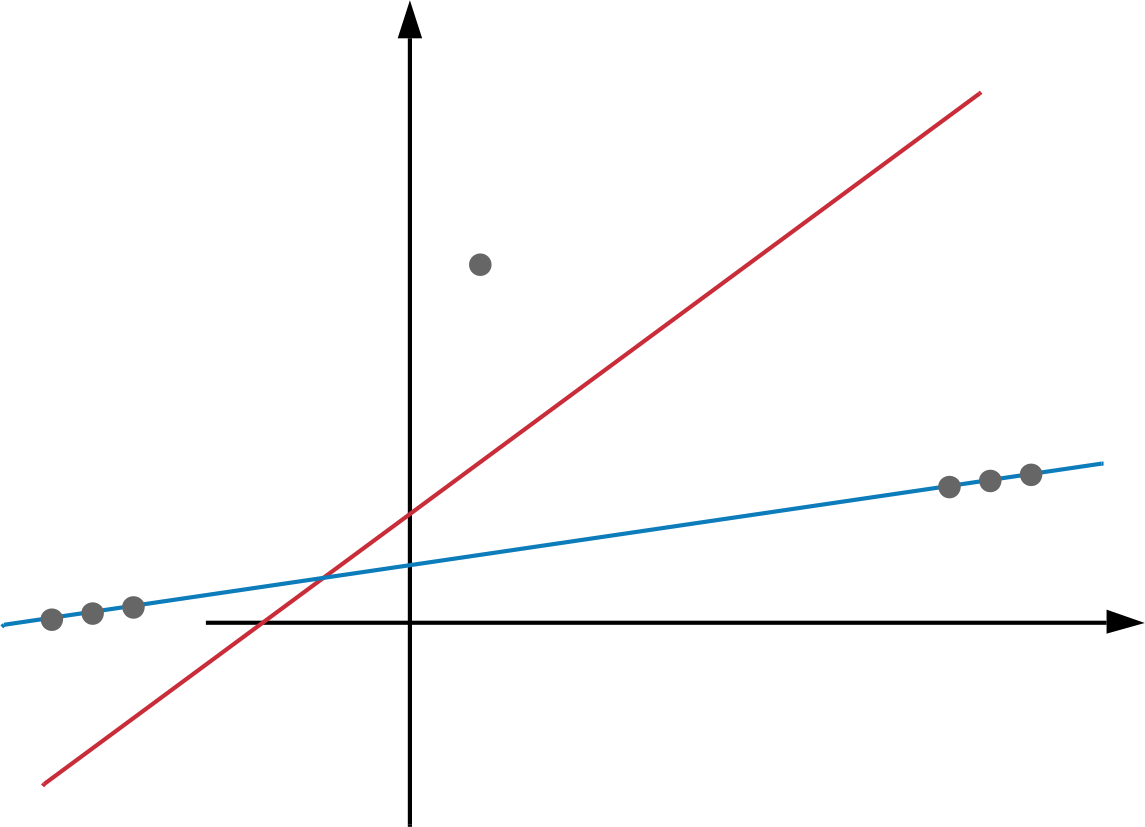
\includegraphics[width=0.4\textwidth]{lossacc.png}
    \caption{Red line has an higher loss but a better accuracy. Instead, blue line has a lower loss but it predicts bad (lower accuracy). We can conclude saying that blue line fits well samples that already known.}
    \label{fig:lossacc}
\end{figure}
Linear Regression has a strange behavior due to the fact that it has not have a sigmoid and the loss MSE works very bad in a classification task without mapping the value in a range.

%TODO: mettere size flatted come input???
\begin{figure}[!h]
    \centering
    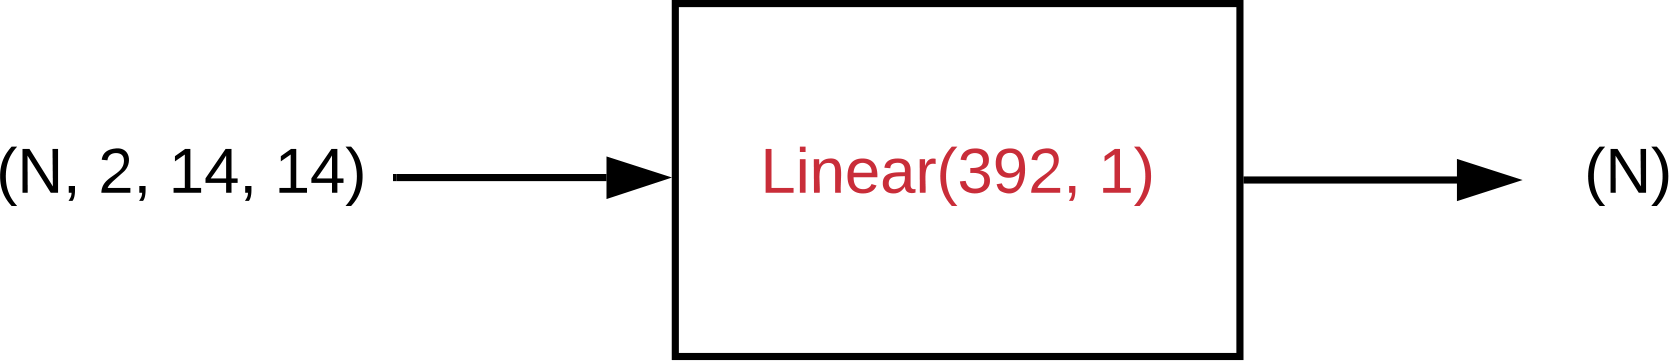
\includegraphics[width=0.4\textwidth]{linearregression.png}
    \caption{Linear Regression model}
    \label{fig:linearregression}
\end{figure}

\begin{figure}[!h]
    \centering
    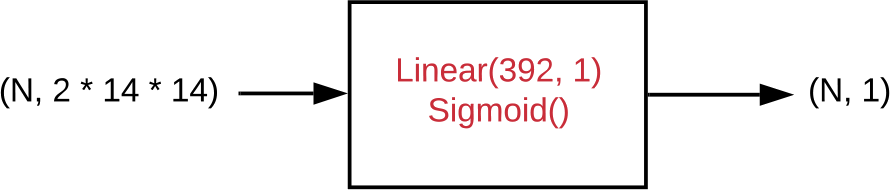
\includegraphics[width=0.4\textwidth]{logistic.png}
    \caption{Logistic Regression model}
    \label{fig:logisticregression}
\end{figure}

\section{Neural Network Models}
\label{sec:nnmodel}
We have implemented two models for the neural network, the first one with 1 loss and the second one with 2 losses, as showed in Fig. \ref{fig:nn1} and Fig. \ref{fig:nn2}. Both models use the same feature extractors but they differs for the classifier. The first one has a boolean classifier that returns 1 if the first image is smaller then the second one. The second model, it has also a digit classifier that returns the corresponding digit for both the handwritten images (we have used an hot encoding to give a target to each node).
%check se img1 < img2 o se era l'inverso!
For these two models the images inputs are passed as 2D images.  Since the feature extractor processes both images together (it does not consider the two images independently), we can use a digit classifier with $20$ nodes as output ($10$ nodes for each images; i.e. from $0$ to $9$ as value of digit). We were expected to have a better result using 2 losses; but since it is a model with just linear layers we could have improved the computation considering both the images independently; we have then decided to try with a convolutional neural network, since \textit{conv3d} allow to automatically process both the images independently. We have observed that two losses could improve the accuracy if the model is more complex, otherwise it would affect negatively the accuracy (as in our case).

% Aggiungere un preprocessing step (flatten nel caso delle reti basate sui layer lineari e niente nel caso della rete conv3d)

\section{Convolutional Neural Network Models}
\label{sec:cnnmodel}
Two models of convolutional neural networks were trained, both received as input 3D images since we have decided to use a \textit{conv3d}. Conv3d are powerful cnn filter that are able to traverse the image in \textit{x}, \textit{y} and \textit{z} axes; that make possible to process both the two images in a independent way. CNN are powerfull since they use pixel locality, then instead of flatting the input as done in previous model we can just consider the 3D raw images. As done, in Sec. \ref{sec:nnmodel} we have decided to compare two models, one with one loss and the other one with two losses, as done with Neural Network models. 
%AGGIUNGERE COMPARAZIONE PER DIRE QUALE DEI DUE MODELLI É STATO MEGLIO
We have used the dropout to generalize better and then obtain a more robust model.

\section{Comparison of models}
\label{sec:comparison}
Since linear models are really sensible to the weights setting 
we have decided to use a unique seed to compare the models.

% #TODO: (REPORT) for 1 to 10 of seed and to plotbox per far vedere outliers --> pensare al codice
% #TODO: (REPORT) fare tabella con num\_params per ogni modello

\section{Conclusion}
\label{sec:conclusion}
As future improvement we would like to implement the cross validation.
%TODO: add
% %%%%%%%%%%%%%%%%%%%%%



% Now we need a bibliography:
\begin{thebibliography}{999}

	%Each item starts with a \bibitem{reference} command and the details thereafter.
	\bibitem{reference0}
    	optim.Adam vs optim.SGD. Let’s dive in.
    	\url{https://medium.com/@Biboswan98/optim-adam-vs-optim-sgd-lets-dive-in-8dbf1890fbdc}
	
% 	\bibitem{reference1}
% 	    Neural networks and deep learning, Michael Nielsen.
	    
%     \bibitem{reference2}
%     Notes of course Deep Learning (EE-559), Prof. François Fleuret.

\end{thebibliography}

% Your document ends here!
\end{document}